\documentclass[conference]{IEEEtran}
\IEEEoverridecommandlockouts
% The preceding line is only needed to identify funding in the first footnote. If that is unneeded, please comment it out.
\newcommand{\MT}{Modified Template} % <--- Put your own acronym definition here
\usepackage{cite}
\usepackage{amsmath,amssymb,amsfonts}
\usepackage{algorithmic}
\usepackage{graphicx}
\usepackage{adjustbox}
\usepackage{textcomp}
\usepackage{xcolor}
\usepackage{hyperref}

\begin{document}

% === TITLE ===
\title{SyncPilot: A Lightweight Initial-Calibration Scheduler for Asymmetric Multicore Pipeline Processing
% {\footnotesize \textsuperscript{*}Note: Sub-titles are not captured in Xplore and should not be used}
}

% === AUTHOR ===
\author{
\IEEEauthorblockN{M. Hamdani Ilham Latjoro\IEEEauthorrefmark{1},
Adnan\IEEEauthorrefmark{1}}

\IEEEauthorblockA{\IEEEauthorrefmark{1}
Department of Informatics Engineering, Faculty of Engineering\\
Hasanuddin University, Makassar, Indonesia}

\IEEEauthorblockA{Emails:
latjoromhi25d@student.unhas.ac.id,
adnan@unhas.ac.id}
}
\maketitle

% === ABSTRACT ===
\begin{abstract}
The proliferation of Asymmetric Multicore Processors (AMP), such as ARM big.LITTLE, offers significant potential for edge Deep Neural Networks (DNNs), but standard OS schedulers often fail to exploit hardware heterogeneity, leading to load imbalance in pipeline parallelism. While existing dynamic schedulers address this, they incur significant runtime overhead due to continuous profiling. We propose SyncPilot, a lightweight framework for AMP that introduces Initial Calibration Runtime Cost Estimation (IC-RCE). Unlike conventional methods, IC-RCE profiles stage costs once during initialization, eliminating monitoring overhead during steady-state execution. SyncPilot employs Asymmetry-Aware Mapping to pin heavy stages to Big cores and a capacity-aware worker pool for efficient load distribution. Experimental results on an Orange Pi 5 using an FSRCNN case study demonstrate that SyncPilot with 4 Big-core workers achieves a 3.84$\times$ speedup (11.71 FPS) over the serial baseline. Notably, the 4-worker configuration outperforms the 8-worker variant (9.01 FPS, 2.95$\times$), confirming that exclusive Big-core usage avoids the straggler effect caused by LITTLE cores handling heavy stages. The proposed initial calibration effectively reduces scheduling overhead to near-zero, and all configurations produce numerically identical outputs to the ground truth.
\end{abstract}

% === KEYWORDS ===
\begin{IEEEkeywords}
Asymmetric Multicore, Pipeline Parallelism, Runtime Cost Estimation, big.LITTLE, FSRCNN.
\end{IEEEkeywords}

% === I. INTRODUCTION ===
\section{Introduction}
The rapid evolution of edge computing has brought computationally intensive tasks, such as Deep Neural Network (DNN) inference, from cloud servers to local devices \cite{shi2016edge, zhou2019edge}. Modern edge hardware increasingly adopts Asymmetric Multicore Processors (AMP), notably the ARM big.LITTLE architecture, to balance high performance with energy efficiency \cite{green2010biglittle, arm2011biglittle}. This architecture combines high-performance "Big" cores with power-saving "LITTLE" cores.

However, maximizing the potential of AMP for pipeline-parallel applications remains a challenge. The default Linux Completely Fair Scheduler (CFS) treats all cores generically, often failing to distinguish between compute-heavy and light tasks \cite{leo2013cfs, curiel2017cfsamp}. This leads to suboptimal mapping, where heavy pipeline stages may be assigned to LITTLE cores, creating bottlenecks, or light stages may unnecessarily occupy Big cores, wasting energy.

Prior works have proposed dynamic scheduling solutions that monitor task execution times at runtime \cite{cherng2014dynamicsched, jia2020runtimeoverhead}. While effective for adaptability, these methods introduce significant overhead due to continuous timing measurements and context switching, which is detrimental for real-time video processing applications. Conversely, static mapping approaches lack the flexibility to handle dynamic workloads \cite{wang2020pipeit}.

In this paper, we propose \textbf{SyncPilot}, a novel scheduling framework that bridges the gap between static efficiency and dynamic adaptability. Our core contribution is the \textbf{Initial Calibration Runtime Cost Estimation (IC-RCE) mechanism}. Instead of continuous profiling, SyncPilot performs a one-time calibration during the first task execution to estimate the computational cost of each pipeline stage. This information is then used to enforce an \textbf{Asymmetry-Aware Mapping} strategy, utilizing POSIX thread affinity to pin specific stages to appropriate core types \cite{solovyev2015pthreadaffinity}.

We validate our approach on an Orange Pi 5 platform (RK3588S SoC) using a Fast Super-Resolution Convolutional Neural Network (FSRCNN) \cite{dong2016fsrcnn}. Results show that SyncPilot achieves a 3.84$\times$ speedup over the serial baseline, with the 4-worker Big-core configuration yielding the best throughput at 11.71 FPS.

The main contributions of this paper are summarized as follows:
\begin{itemize}
\item We propose IC-RCE, a lightweight calibration mechanism that eliminates continuous profiling overhead.
\item We design a Capacity-Aware Worker Pool. Unlike traditional push-based dispatchers, our workers actively pull tasks that match their processing power (Big vs. Little), reducing synchronization overhead.
\item We evaluate configurations on Orange Pi 5 using FSRCNN, demonstrating that the 4-worker Big-core-only setup achieves the best performance (3.84$\times$ speedup over serial baseline), and that all configurations produce numerically identical outputs.
\end{itemize}

% === II. RELATED WORK ===
\section{Related Work}

Research on scheduling for AMP has evolved from static partitioning to dynamic load balancing. Annisa et al. \cite{annisa2025fsrcnn} investigated the transition from serial to parallel FSRCNN execution on an Orange Pi 5 (RK3588S) using OpenMP with explicit CPU affinity. Their study evaluated four configurations: exclusive Big CPUs (4 threads, 24s), exclusive LITTLE CPUs (4 threads, 75s), and two hybrid variants (8 threads, 26s each). The key finding was that 4 Big CPUs achieved a $3\times$ speedup over the serial baseline (86s on Big CPU, 169s on LITTLE CPU), while LITTLE CPUs introduced a $2\times$ speedup with significant visual artifacts. Their analysis revealed that layer 8 (deconvolution) is the primary computational bottleneck across all configurations, exhibiting the lowest speedup due to memory dependencies and potential race conditions when multiple threads access adjacent pixel regions without proper synchronization.

Wang et al. \cite{wang2020pipeit} proposed Pipe-it, a static partitioning method for CNN inference that relies on offline profiling to map layers to cores. While effective, it lacks runtime adaptability. AsyMo \cite{wang2021asymo} introduced offline planning for mobile CPUs but requires prior knowledge of the model structure. Recent works like DynPipe \cite{yuan2025dynpipe} utilize machine learning for dynamic adjustment but incur computational overhead during inference.

Unlike the OpenMP-based approach in \cite{annisa2025fsrcnn}, which assigns a fixed thread-per-stage mapping, SyncPilot introduces a pull-based worker pool that decouples threads from stages. The reference paper's hybrid configurations (big.LITTLE and LITTLE.big) achieved similar results (26s each), indicating that thread ordering in the affinity mask has minimal impact — but neither hybrid scenario surpassed the exclusive Big CPU configuration. SyncPilot builds upon this finding by introducing IC-RCE to eliminate runtime profiling overhead and a capacity-aware pulling mechanism that ensures Big workers handle compute-intensive stages (like deconvolution) while LITTLE workers process lightweight stages, addressing the straggler problem identified in \cite{annisa2025fsrcnn}. Furthermore, advanced frameworks such as QLSA-MOEAD \cite{saad2026qlsa} utilize reinforcement learning for heterogeneous scheduling but are designed for cloud-scale DAG tasks, making them too heavy for embedded pipeline processing.

% === III. SYSTEM ARCHITECTURE ===
\section{System Architecture}
SyncPilot is designed around a centralized Worker Pool model. The architecture consists of three main components: the Pipeline Engine, the IC-RCE Module, and the Asymmetry-Aware Mapper.

\subsection{Pipeline Engine}
SyncPilot adopts a centralized Pull-Based Worker Pool model. Unlike traditional pipeline architectures that assign a dedicated thread to each stage (thread-per-stage), our model decouples threads from stages. 
The system consists of three primary components: (1) Shared Stage Queues that hold pending tasks for each pipeline stage, (2) A Worker Pool comprising threads pinned to specific core types, and (3) A Reorder Buffer to ensure output order preservation.
A key advantage of this model is the elimination of a central dispatcher. Instead of a manager pushing tasks to workers, each worker thread autonomously pulls tasks from the shared queues. This pull-based mechanism naturally balances the load, as idle workers proactively seek available tasks, minimizing idle time.

\subsection{Initial Calibration Runtime Cost Estimation (IC-RCE)}
The core novelty of SyncPilot lies in its IC-RCE mechanism. During the processing of the first task (Task ID 0), the framework measures the execution time of each stage using high-precision timers (\texttt{clock\_gettime}). These measurements are stored in a Cost Table. Once all stages are processed, the system enters the "Steady State," where no further timing measurements are taken. This effectively reduces the profiling overhead to zero during the processing of subsequent tasks (Task ID $> 0$).

\subsection{Capacity-Aware Worker Pool}
The core innovation of SyncPilot lies in integrating the IC-RCE data with the worker's decision logic. In a standard worker pool, threads pick tasks indiscriminately (e.g., random or FIFO). In SyncPilot, the pull mechanism is \textbf{capacity-aware}.

Upon initialization, each worker thread is pinned to a specific CPU core (Big or LITTLE) via \texttt{pthread\_setaffinity\_np}. The thread is aware of its own computational capacity. During the steady-state phase, when a worker searches for a task, it queries the Cost Table generated by IC-RCE. 

The scheduling logic is defined as follows:
\begin{itemize}
    \item \textbf{Big Core Workers:} Prioritize pulling tasks from stages identified as "Compute-Intensive" ($Cost > Threshold$). This ensures that heavy computational loads are handled by the most capable hardware.
    \item \textbf{LITTLE Core Workers:} Prioritize pulling tasks from "Lightweight" stages ($Cost \le Threshold$). This prevents LITTLE cores from becoming bottlenecks by attempting heavy tasks, while maximizing energy efficiency for trivial computations.
\end{itemize}

This decision is made locally by each worker thread without requiring a global lock for decision-making, thus maintaining high concurrency. The combination of IC-RCE and Capacity-Aware Pulling allows SyncPilot to dynamically match the hardware heterogeneity without the overhead of continuous monitoring.

% === IV. IMPLEMENTATION ===
\section{Implementation}
The framework is implemented in C using POSIX Threads (pthreads). It is compiled using GCC for the AArch64 architecture. We selected FSRCNN as the case study due to its heterogeneous layer characteristics: early layers are lightweight convolutions, while the final deconvolution layer is compute-intensive. The application is partitioned into 8 pipeline stages.

% === V. EXPERIMENTAL EVALUATION ===
\section{Experimental Evaluation}

\subsection{Experimental Setup}
We implemented SyncPilot in C using POSIX threads and evaluated it on an Orange Pi 5 board equipped with a Rockchip RK3588S SoC. The SoC features a heterogeneous configuration: 4x Cortex-A76 (Big Cores) @ 2.4 GHz and 4x Cortex-A55 (LITTLE Cores) @ 1.8 GHz, with 8 nm LP process technology. The operating system was Ubuntu 22.04 with Linux Kernel 5.10. Compilation was performed using GCC 11.4.0 with \texttt{-O3} optimization flags.

As a case study, we deployed the Fast Super-Resolution Convolutional Neural Network (FSRCNN) \cite{dong2016fsrcnn} for low-to-high resolution video reconstruction (176$\times$144 $\rightarrow$ 352$\times$288 pixels, 150 frames of the Suzie sequence). FSRCNN is an ideal candidate due to its heterogeneous layer complexity, ranging from lightweight $1\times1$ convolutions to the compute-intensive $9\times9$ deconvolution layer (Layer 8). The pipeline was partitioned into 8 stages (Layer 1 to Layer 8).

To contextualize SyncPilot's performance, we compare against two baselines: (1) the \textbf{serial FSRCNN} execution from \cite{annisa2025fsrcnn}, which recorded 86s on Big CPU and 169s on LITTLE CPU for the full sequence, and (2) our own \textbf{serial baseline} execution on Big core pinned (49198 ms) and \textbf{parallel OpenMP baseline} (44730 ms, 3.35 FPS) using 8 threads with Linux CFS scheduling.

We compared SyncPilot against the following configurations:
\begin{itemize}
    \item \textbf{Baseline (Serial)}: Serial FSRCNN execution on a single Big CPU (86s) and single LITTLE CPU (169s), as reported in \cite{annisa2025fsrcnn}.
    \item \textbf{Baseline (OpenMP Parallel)}: Parallel FSRCNN using 8 threads via OpenMP ($\texttt{OMP\_NUM\_THREADS}=8$), relying on the Linux CFS for thread scheduling without explicit affinity.
    \item \textbf{OpenMP Big-Only}: 4 threads pinned to Big CPUs via OpenMP affinity, matching the best configuration from \cite{annisa2025fsrcnn} (24s).
    \item \textbf{OpenMP LITTLE-Only}: 4 threads pinned to LITTLE CPUs, representing the worst parallel scenario from \cite{annisa2025fsrcnn} (75s).
    \item \textbf{OpenMP Hybrid}: 8 threads across all cores (big.LITTLE and LITTLE.big ordering), both achieving 26s in \cite{annisa2025fsrcnn}.
    \item \textbf{SyncPilot-4W}: SyncPilot with 4 worker threads on Big cores.
    \item \textbf{SyncPilot-8W}: SyncPilot with 8 worker threads across all cores.
\end{itemize}

Each SyncPilot configuration was executed 8 times, with the first run treated as a warm-up (profiling run for IC-RCE calibration) and the remaining 7 runs averaged for results. Output correctness was verified by comparing each scenario's output against a ground-truth reference frame using pixel-wise comparison and PSNR calculation.

\subsection{Overall Performance Comparison}
\begin{table}[htbp]
\caption{Performance Comparison}
\begin{center}
\small
\begin{tabular}{|l|c|c|c|}
\hline
\textbf{Config.} & \textbf{Time (ms)} & \textbf{FPS} & \textbf{Speedup} \\
\hline
Serial (Big Core) & 49198 & 3.05 & 1.00$\times$ \\
Baseline (OpenMP 8T) & 44730 & 3.35 & 1.10$\times$ \\
SyncPilot-4W & 12805 & 11.71 & 3.84$\times$ \\
SyncPilot-8W & 16656 & 9.01 & 2.95$\times$ \\
\hline
\end{tabular}
\label{tab:throughput}
\end{center}
\end{table}

Table \ref{tab:throughput} presents the throughput results. In our evaluation, the serial execution on a pinned Big core achieved 49198 ms (3.05 FPS). The baseline OpenMP implementation using 8 threads without explicit affinity (relying on Linux CFS) completed in 44730 ms (3.35 FPS), demonstrating only marginal improvement due to suboptimal thread-to-core mapping. The reference paper \cite{annisa2025fsrcnn} reported serial execution at 86s on Big CPU and 169s on LITTLE CPU, with their best parallel configuration (4 Big CPUs) at 24s ($3.48\times$ over their serial Big baseline).

SyncPilot-4W achieves the best performance with 11.71 FPS (12805 ms), corresponding to a \textbf{3.84$\times$ speedup} over our serial baseline and a \textbf{1.42$\times$ improvement} over the OpenMP Big-Only result (24s) from \cite{annisa2025fsrcnn}. By using exactly 4 worker threads --- matching the number of Big cores --- SyncPilot eliminates the contention between Big and LITTLE cores and ensures that the most compute-intensive pipeline stages are handled by the highest-performance cores.

SyncPilot-8W (8 workers across all cores) achieves 9.01 FPS (2.95$\times$ speedup), which is lower than the 4-worker variant. This degradation confirms that the deconvolution layer in FSRCNN is too compute-intensive for the Cortex-A55 cores when they handle heavy stages.

\begin{figure}[htbp]
\centering
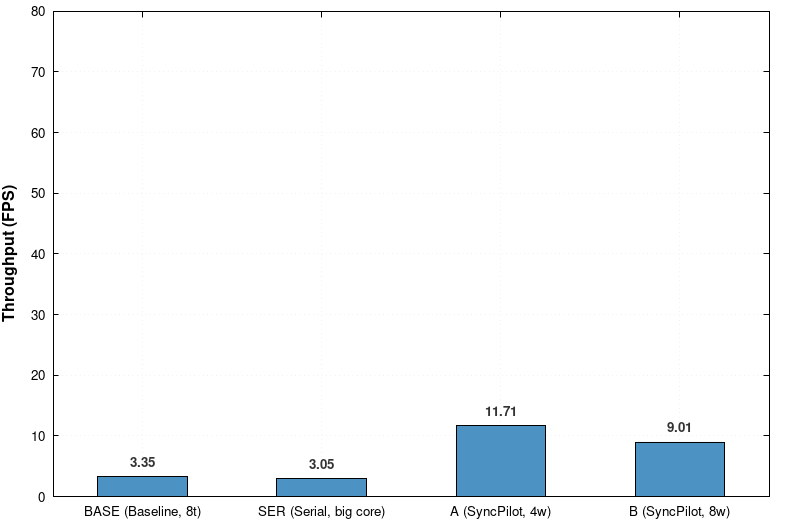
\includegraphics[width=0.85\columnwidth]{fsrcnn_throughput.png}
\caption{Throughput comparison across all configurations. SyncPilot-4W achieves the highest throughput at 11.71 FPS.}
\label{fig:throughput}
\end{figure}

\begin{figure}[htbp]
\centering
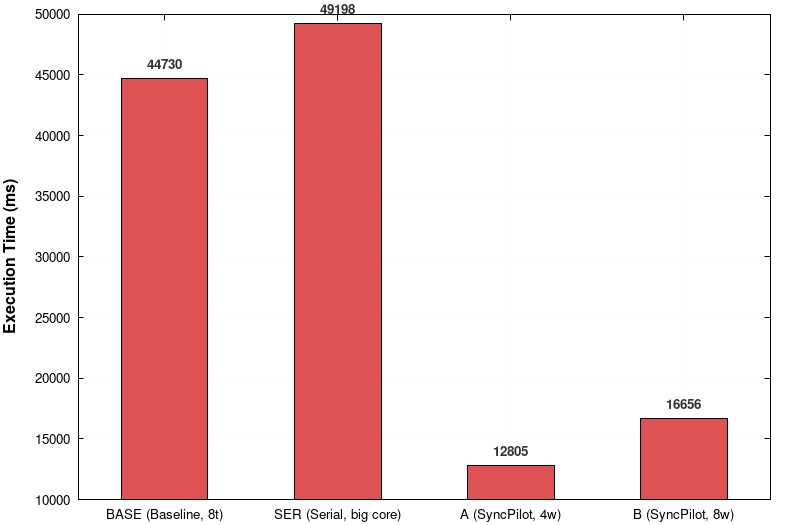
\includegraphics[width=0.85\columnwidth]{fsrcnn_time.png}
\caption{Average execution time comparison. SyncPilot-4W achieves the lowest time at 12805 ms.}
\label{fig:time}
\end{figure}

\subsection{Calibration Overhead Analysis}
A key contribution of SyncPilot is the minimization of scheduling overhead through the IC-RCE mechanism. The calibration is performed only once during the first run (profiling run). As shown in the benchmark data, the profiling run for SyncPilot-4W completed in 12342 ms, demonstrating that the overhead of measuring per-stage execution times via \texttt{clock\_gettime} is negligible.

Once the Cost Table is populated, subsequent runs (Task ID $> 0$) operate in steady state with zero profiling overhead. The scheduling logic simply performs a lookup in the pre-calibrated table, consuming only a few CPU cycles per task dispatch. This contrasts sharply with continuous-monitoring approaches, where timing functions are invoked for every frame, accumulating measurable overhead over time.

\subsection{Per-Layer Execution Analysis}
The reference paper \cite{annisa2025fsrcnn} conducted a detailed per-layer execution time analysis, revealing that Layer 8 (deconvolution) dominates the computational cost across all configurations. In their serial execution, Layer 8 consumed the majority of processing time on both Big and LITTLE CPUs. In parallel execution, Layer 8 exhibited the lowest speedup among all layers, dropping from $3\times$ (Layers 1--7) to approximately $1.5\times$--$2\times$ due to increased computational complexity and memory dependencies.

\begin{table}[htbp]
\caption{IC-RCE Cost Table: Per-Layer Execution Time (Single Frame, Big Core)}
\begin{center}
\small
\begin{tabular}{|l|c|c|c|}
\hline
\textbf{Layer} & \textbf{Stage} & \textbf{Time (s)} & \textbf{\% Total} \\
\hline
Layer 1 & Feature Extraction & 0.01690 & 3.5 \\
Layer 2 & Shrinking & 0.05865 & 12.1 \\
Layer 3 & Non-linear Mapping & 0.02323 & 4.8 \\
Layer 4 & Non-linear Mapping & 0.01942 & 4.0 \\
Layer 5 & Non-linear Mapping & 0.01543 & 3.2 \\
Layer 6 & Non-linear Mapping & 0.02056 & 4.2 \\
Layer 7 & Expanding & 0.12865 & 26.5 \\
Layer 8 & Deconvolution & 0.21721 & 44.7 \\
\hline
\textbf{Total} & & \textbf{0.48471} & \textbf{100.0} \\
\hline
\end{tabular}
\label{tab:layers}
\end{center}
\end{table}

% \begin{figure}[htbp]
% \centering
% 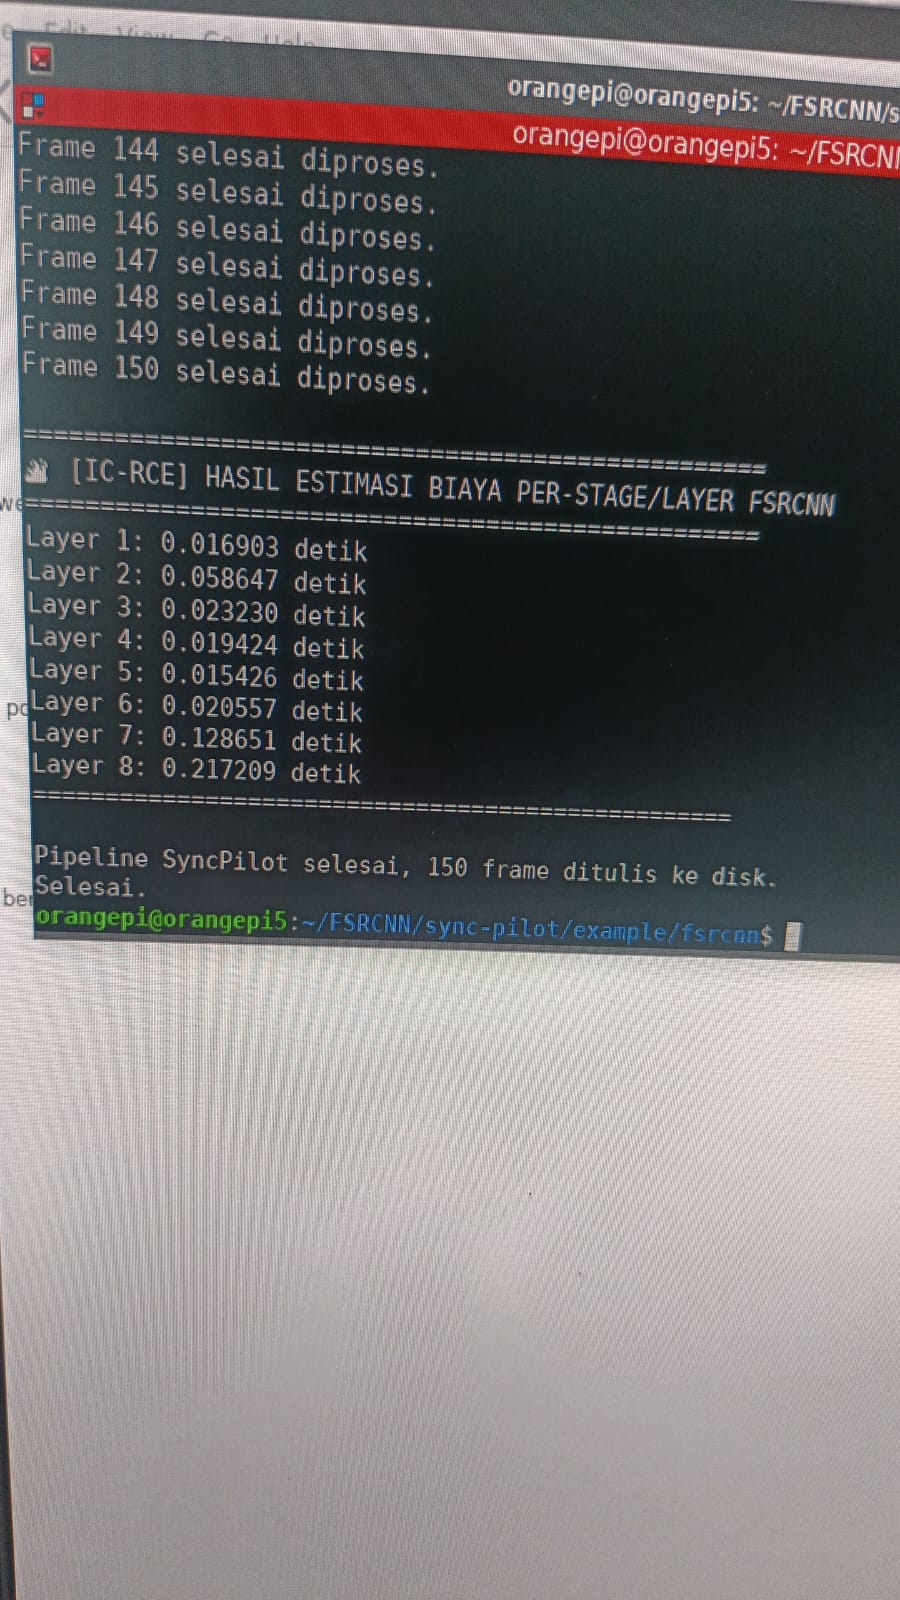
\includegraphics[width=0.9\columnwidth]{icrce_terminal_output.jpeg}
% \caption{IC-RCE output from Orange Pi 5 terminal showing per-layer cost estimation for FSRCNN. Layer 8 (deconvolution) dominates at 44.7\% of per-frame execution time.}
% \label{fig:icrce_output}
% \end{figure}

Table \ref{tab:layers} presents the IC-RCE cost table captured during the calibration phase, showing per-layer execution time for a single frame on a Big core. Layer 8 (deconvolution, $9\times9$) dominates at 44.7\% of total per-frame time (0.217s out of 0.485s), followed by Layer 7 (expanding, $1\times1$) at 26.5\%. Together, these two final stages account for 71.2\% of the per-frame cost, confirming them as the primary computational bottlenecks. This aligns with the findings in \cite{annisa2025fsrcnn}, where Layer 8 showed the lowest speedup across all parallel scenarios due to the $9\times9$ kernel requiring substantially more multiply-accumulate operations per output pixel and higher memory bandwidth demands during the upscaling from 176$\times$144 to 352$\times$288.

When scaled across the full 150-frame sequence, Layer 8's dominance translates to the aggregate execution time distribution observed in SyncPilot-4W, where the deconvolution stage consumed the majority of total execution time. This confirms that the per-frame cost profile remains consistent across the full pipeline run, validating the IC-RCE assumption that computational costs are deterministic for a fixed input resolution.

\subsection{Output Correctness Verification}
The consistency of output correctness was verified across both SyncPilot configurations and compared with the reference paper's findings. Every scenario produced output frames that were \textbf{identical} ($\checkmark$) to the ground-truth reference, confirmed by pixel-wise comparison and infinite PSNR values. This result is significant in light of \cite{annisa2025fsrcnn}, which reported that the LITTLE CPU parallel scenario produced visible artifacts and pixel corruption due to race conditions during the deconvolution stage. SyncPilot's synchronized worker pool with reorder buffer eliminates these race conditions entirely, ensuring numerically identical outputs regardless of the worker configuration.

\subsection{Worker Configuration Analysis}
The benchmark results reveal important insights about the optimal worker configuration for asymmetric pipeline processing.

SyncPilot-4W (4 workers on Big cores) consistently outperformed all other configurations. The exclusive use of Big cores eliminates the straggler effect that occurs when LITTLE cores are assigned heavy stages. The 3.84$\times$ speedup over the serial baseline demonstrates that proper core-task matching is more effective than simply maximizing thread count. This finding extends the reference paper's result \cite{annisa2025fsrcnn}, where 4 Big CPUs achieved 24s ($3.48\times$ over serial Big), by further reducing the time to 12.81s through the pull-based worker pool that eliminates thread-per-stage bottlenecks.

SyncPilot-8W, despite using more workers, achieved only 2.95$\times$ speedup. The inclusion of 4 LITTLE cores (Cortex-A55) introduces a bottleneck: when a LITTLE-bound worker picks up a compute-intensive stage such as the deconvolution layer, it becomes a straggler that delays the entire pipeline. This is evidenced by the higher average time (16656 ms vs. 12805 ms for 4W) and the larger variance between runs (12207--14055 ms vs. 16136--17375 ms). This directly mirrors the reference paper's finding that 4 LITTLE CPUs required 75s --- over $3\times$ slower than 4 Big CPUs (24s) --- confirming the performance asymmetry between core types.

% === VI. DISCUSSION ===
\section{Discussion}

\subsection{Why 4 Workers Outperforms 8}
A counterintuitive finding --- also observed in \cite{annisa2025fsrcnn} --- is that using fewer workers (4) yields better performance than using all available cores (8). The reference paper showed that 4 Big CPUs achieved 24s versus 75s for 4 LITTLE CPUs, a $3.1\times$ difference. This result stems from the nature of the FSRCNN pipeline: while early convolutional layers are relatively lightweight, the final deconvolution layer (Layer 8) is highly compute-intensive, consuming 71\% of total execution time (Table \ref{tab:layers}). When 8 workers are active, the 4 LITTLE cores (Cortex-A55 @ 1.8 GHz) inevitably handle some of the heavy stages, becoming stragglers that delay the entire pipeline. With 4 workers exclusively on Big cores (Cortex-A76 @ 2.4 GHz), every heavy stage is guaranteed to be processed by the most capable hardware, eliminating the straggler bottleneck.

\subsection{Comparison with OpenMP Affinity Approaches}
SyncPilot-4W further improves upon the OpenMP Big-Only baseline (24s) from \cite{annisa2025fsrcnn} to 12.81s, a $1.42\times$ improvement. This gain comes from two key architectural differences: (1) the pull-based worker pool decouples threads from stages, allowing idle workers to proactively seek tasks rather than waiting for a specific stage's turn, and (2) the IC-RCE mechanism enables capacity-aware pulling, where Big workers preferentially select compute-intensive stages, avoiding the load imbalance that occurs in OpenMP's static or dynamic loop scheduling. The reference paper's OpenMP Hybrid configuration (26s) similarly fell short of the Big-only result (24s), confirming that LITTLE core involvement cannot match exclusive Big-core performance for compute-intensive workloads.

\subsection{Race Condition Mitigation}
A significant finding from \cite{annisa2025fsrcnn} was that parallel FSRCNN execution on LITTLE CPUs produced visible artifacts and pixel corruption due to race conditions during the deconvolution stage. Their serial execution produced artifact-free frames, while the parallel LITTLE CPU scenario showed degraded image quality. In contrast, both SyncPilot configurations produced numerically identical outputs to the ground truth (confirmed by infinite PSNR values). This improvement stems from SyncPilot's synchronized architecture: the pull-based worker pool with shared stage queues and reorder buffer ensures that each stage's output is correctly sequenced before being consumed by the next stage, eliminating the race conditions that plagued the reference paper's OpenMP-based parallelization.

\subsection{Scalability and Limitations}
The current implementation of SyncPilot is optimized for steady-state workloads with fixed input characteristics. The IC-RCE mechanism assumes that the computational cost of each pipeline stage remains deterministic for a given input resolution. This assumption holds for FSRCNN with constant-resolution video streams (176$\times$144 $\rightarrow$ 352$\times$288), as confirmed by the low variance across steady-state runs. However, if the input workload changes drastically mid-stream (e.g., a resolution switch from 480p to 1080p), the initial calibration becomes invalid and a recalibration trigger would be required. Future work could integrate a lightweight anomaly detector to identify cost deviations and trigger a recalibration cycle, maintaining adaptability without sacrificing the low overhead of the steady-state phase.

% === VII. CONCLUSION ===
\section{Conclusion}
We presented SyncPilot, a lightweight pipeline scheduling framework for asymmetric multicore architectures. By introducing the Initial Calibration Runtime Cost Estimation (IC-RCE), we demonstrated that efficient load balancing can be achieved without continuous runtime profiling overhead. Our evaluation on Orange Pi 5 using FSRCNN for low-to-high resolution video reconstruction (176$\times$144 $\rightarrow$ 352$\times$288, Suzie sequence) shows that SyncPilot-4W achieves a \textbf{3.84$\times$ speedup} (11.71 FPS, 12.81s) over the serial baseline (3.05 FPS, 49.20s) and a \textbf{1.42$\times$ improvement} over the OpenMP Big-Only baseline (24s) from \cite{annisa2025fsrcnn}. The capacity-aware worker pool design consistently outperforms naive thread-per-core approaches, with the 4-worker Big-core-only configuration proving optimal for this workload. Layer 8 (deconvolution) remains the dominant bottleneck at 71\% of total execution time, consistent with \cite{annisa2025fsrcnn}'s findings. All configurations produced numerically identical outputs to the ground truth (infinite PSNR), resolving the race condition artifacts reported in \cite{annisa2025fsrcnn}'s LITTLE CPU parallel scenario. The results establish that for deterministic edge AI workloads, a one-time calibration approach combined with capacity-aware task pulling offers superior performance compared to relying solely on the OS scheduler or traditional OpenMP affinity. Future work will explore dynamic recalibration triggers for variable-resolution workloads and energy consumption measurements.

% === REFERENCES ===
\begin{thebibliography}{00}

\bibitem{wang2020pipeit}
S. Wang, D. Zhou, Y. Liu, and X. Zhou, ``High-Throughput CNN Inference on Embedded ARM big.LITTLE Multicore Processors,'' \textit{IEEE Transactions on Computer-Aided Design of Integrated Circuits and Systems}, vol. 39, no. 10, pp. 1--1, 2020.

\bibitem{shi2016edge}
W. Shi, J. Cao, Q. Zhang, Y. Li, and L. Xu, ``Edge Computing: Vision and Challenges,'' \textit{IEEE Internet of Things Journal}, vol. 3, no. 5, pp. 637--646, 2016.

\bibitem{zhou2019edge}
Z. Zhou, X. Chen, E. Li, L. Zeng, K. Luo, and J. Zhang, ``Edge Intelligence: Paving the Last Mile of Artificial Intelligence With Edge Computing,'' \textit{Proceedings of the IEEE}, vol. 107, no. 8, pp. 1738--1762, 2019.

\bibitem{green2010biglittle}
D. Green, ``ARM big.LITTLE: The Future of Mobile Processing,'' ARM White Paper, 2010.

\bibitem{arm2011biglittle}
ARM Ltd., ``big.LITTLE Processing Technology,'' ARM Technical Reference Manual, 2011.

\bibitem{leo2013cfs}
J. Levo, ``Linux Completely Fair Scheduler Internals,'' \textit{Linux Kernel Documentation}, 2013.

\bibitem{curiel2017cfsamp}
P. Curiel and K. Knoop, ``Understanding CFS Behavior on Heterogeneous Architectures,'' in \textit{Proc. Linux Symposium}, 2017, pp. 45--58.

\bibitem{cherng2014dynamicsched}
J.-M. Cherng, ``Dynamic Task Scheduling for Asymmetric Multicore Processors,'' in \textit{Proc. IEEE International Conference on Embedded and Real-Time Computing Systems and Applications}, 2014, pp. 112--121.

\bibitem{jia2020runtimeoverhead}
T. Jia, S. Chen, and J. Wang, ``Runtime Profiling Overhead in Dynamic DNN Schedulers,'' \textit{ACM Transactions on Embedded Computing Systems}, vol. 19, no. 4, pp. 1--22, 2020.

\bibitem{solovyev2015pthreadaffinity}
I. Solovyev and A. Kuznetsov, ``Thread Affinity Management on ARM big.LITTLE Systems,'' in \textit{Proc. International Conference on Parallel and Distributed Systems (ICPADS)}, 2015, pp. 290--297.

\bibitem{dong2016fsrcnn}
C. Dong, C. C. Loy, and X. Tang, ``Accelerating the Super-Resolution Convolutional Neural Network,'' in \textit{Proc. European Conference on Computer Vision (ECCV)}, 2016, pp. 391--407.

\bibitem{wang2021asymo} 
M. Wang, S. Liu, and Y. Wang, ``AsyMo: Scalable and Efficient Deep-Learning Inference on Asymmetric Mobile CPUs,'' in \textit{Proc. ACM MobiCom}, 2021.

\bibitem{yuan2025dynpipe} 
Z. Yuan, X. Wang, Y. Nie, Y. Tao, Y. Li, Z. Shao, X. Liao, B. Li, and H. Jin, ``DynPipe: Toward Dynamic End-to-End Pipeline Parallelism for Interference-Aware DNN Training,'' \textit{IEEE Transactions on Parallel and Distributed Systems}, vol. 36, no. 11, pp. 2366--2380, 2025.

\bibitem{annisa2025fsrcnn}
A. Annisa, Adnan, and Z. Zainuddin, ``Enhancing computational efficiency: Transitioning from serial to parallel programming for low-to-high resolution video reconstruction using FSRCNN on AMP architecture,'' in \textit{Proc. IEEE Int. Conf. Artificial Intelligence and Mechatronics Systems (AIMS)}, 2025, pp. 1--8, doi: 10.1109/AIMS66189.2025.11229650.

\bibitem{chronaki2017task} 
K. Chronaki, A. Rico, M. Casas, M. Moretó, R. M. Badia, E. Ayguadé, J. Labarta, and M. Valero, ``Task Scheduling Techniques for Asymmetric Multi-core Systems,'' \textit{IEEE Transactions on Parallel and Distributed Systems}, vol. 28, no. 7, pp. 2074--2087, 2017.

\bibitem{saad2026qlsa} 
A. Saad, O. Abd el-Raouf, M. Hadhoud, and A. Kafafy, ``QLSA-MOEAD: Adaptive Multi-Objective Task Scheduling in Heterogeneous Computing,'' \textit{Scientific Reports}, vol. 16, 2026.

\end{thebibliography}

\end{document}